%%%%%%%%%%%%%%%%%%%%%%%%%%%%%%%%%%%%%%%%%%%%%%%%%%%%%%%%%%%%%%%%%%%%%%%%%%%%%%%%
\section{Experiments}\label{sec:face_flow_experiments}
%%%%%%%%%%%%%%%%%%%%%%%%%%%%%%%%%%%%%%%%%%%%%%%%%%%%%%%%%%%%%%%%%%%%%%%%%%%%%%%%
In this section, we describe the set of qualitative and quantitative experiments
that we conducted in order to demonstrate the effectiveness of our proposed algorithm,
``Face Flow''. We concentrate on two scenarios: firstly we measure the effectiveness
of the basis learnt via optical flow and compare it's performance against
a number of state-of-the-art optical methods. This is a fair comparison as our
basis was also acquired from optical flow. Secondly, we investigate the use
of our basis learnt using a 3D statistical model in computing correspondences
for a sequence containing pose and expression. We use these required 2D correspondences
and the prior correspondence of our model with the 3D basis in order to recover
dense 3D shape for the sequence. We compare this shape to that recovered from
a set of 68 sparse annotations, which is the standard methodology used for recovering
shape using facial landmarks at the moment.

In order to verify that our method is competitive with the state-of-the-art
optical flow methods,
we compared against the algorithms of
\citet{garg2013variational} (denoted MFSF),
\citet{revaud2015epicflow} (denoted EPICFlow),
\citet{liu2011sift} (denoted SIFTFlow) and the large displacement
optical method of \citet{brox2011large} (denoted LDOF). We also provide two
formulations of our method, one which enforces the low-rank constraint on the coefficients
and one which does not. The latter corresponds to the choice of $\lambda=k$.
We denote these two methods Face Flow Low-Rank (LR) and Face Flow
Full-Rank (FR). This self evaluation is particularly useful for demonstrating the importance
and effectiveness of the low-rank constraint for multi-frame facial flow.

To quantitatively evaluate the optical flow model for Face Flow, 
we propose a novel ground truth dataset formed
from facial motion capture data~\cite{zhang2004spacetime}. The sequence that we
evaluate must be in correspondence and ideally contain an interesting
sequence of deformations. Performance capture data is ideal for this purpose, as
it is necessarily in correspondence and often deals with actors portraying
scripted, emotional content. We also evaluate Face Flow on a realistic sequence
portraying a number of common issues in facial videos, including motion blur
and occlusions.

In order to improve the robustness of our algorithm, we adopt a pseudo coarse-to-fine
strategy for basis construction and create three bases of increasing scale. This is also
commonly employed within optical algorithms to improve robustness. 
In all of the following experiments, the feature descriptor employed is the dense 
SIFT~\cite{lowe2004distinctive} feature provided by VlFeat~\cite{vedaldi08vlfeat}.
%%%%%%%%%%%%%%%%%%%%%%%%%%%%%%%%%%%%%%%%%%%%%%%%%%%%%%%%%%%%%%%%%%%%%%%%%%%%%%%%
\subsection{Practical Deformation Basis Construction}\label{subsec:face_flow_experiments_basis}
%%%%%%%%%%%%%%%%%%%%%%%%%%%%%%%%%%%%%%%%%%%%%%%%%%%%%%%%%%%%%%%%%%%%%%%%%%%%%%%%
%%%%%%%%%%%%%%%%%%%%%%%%%%%%%%%%%%%%%%%%
\setlength{\tabcolsep}{2pt}
\begin{figure}
    \centering
    \resizebox{\textwidth}{!}{%
    \begin{tabular}{cccccc}
    Mean &  PC 1 & PC 2 & PC 3 & PC 4 & PC 5 \\
    \multirow{2}{*}{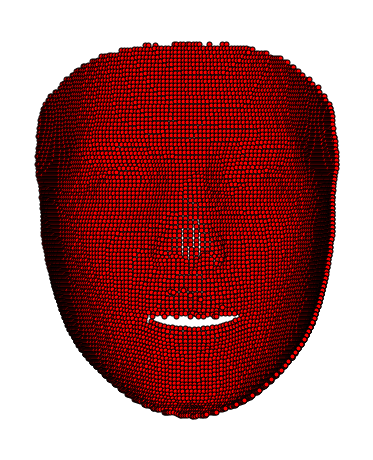
\includegraphics[valign=m,scale=0.16]{face_flow/images/3d_pca_basis/mean}} &  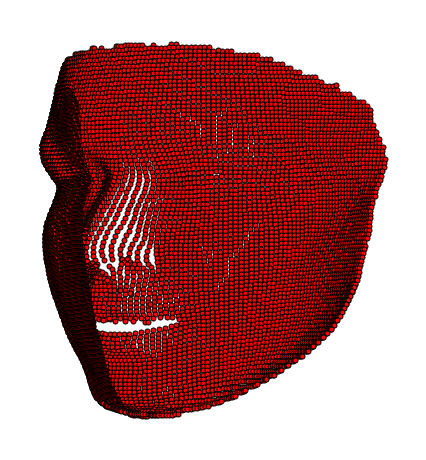
\includegraphics[valign=m,scale=0.16]{face_flow/images/3d_pca_basis/0_plus2} & 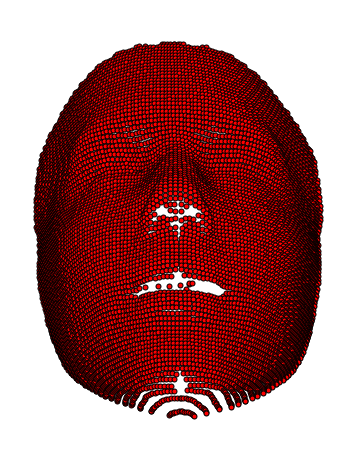
\includegraphics[valign=m,scale=0.16]{face_flow/images/3d_pca_basis/1_plus2} & 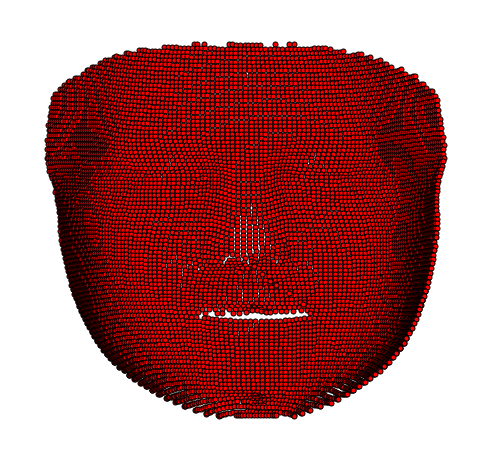
\includegraphics[valign=m,scale=0.16]{face_flow/images/3d_pca_basis/2_plus2} & 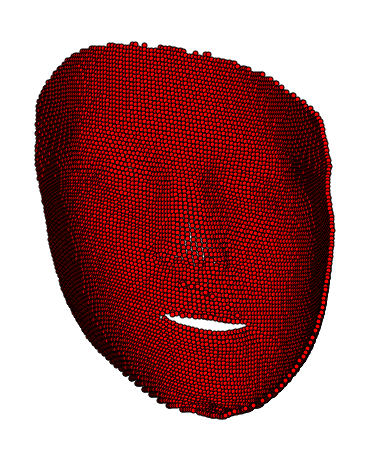
\includegraphics[valign=m,scale=0.16]{face_flow/images/3d_pca_basis/3_plus2} & 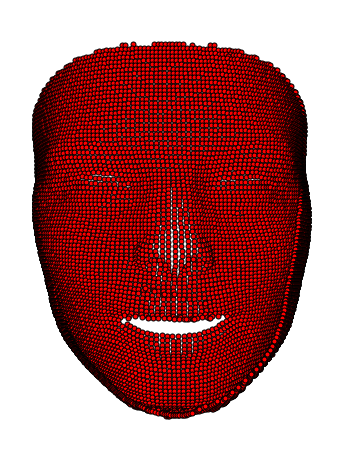
\includegraphics[valign=m,scale=0.16]{face_flow/images/3d_pca_basis/4_plus2} \\
     & 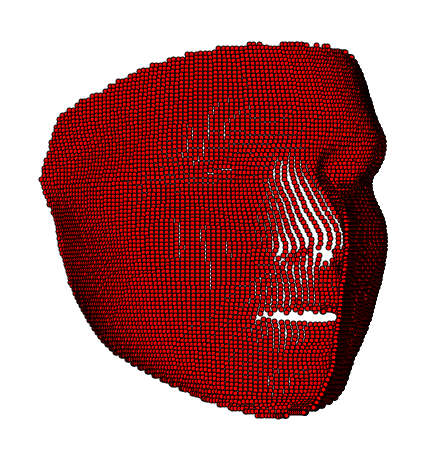
\includegraphics[valign=m,scale=0.16]{face_flow/images/3d_pca_basis/0_minus2} & 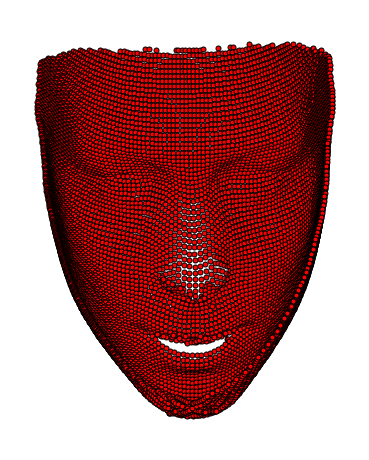
\includegraphics[valign=m,scale=0.16]{face_flow/images/3d_pca_basis/1_minus2} & 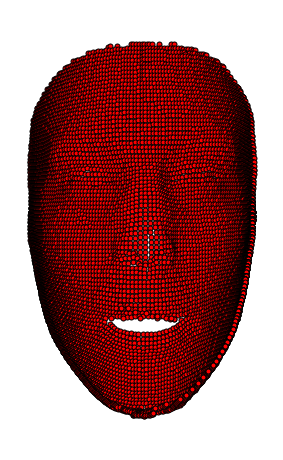
\includegraphics[valign=m,scale=0.16]{face_flow/images/3d_pca_basis/2_minus2} & 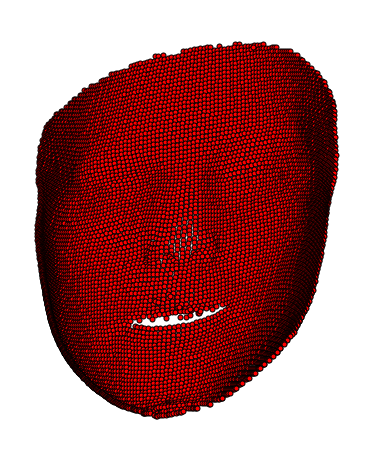
\includegraphics[valign=m,scale=0.16]{face_flow/images/3d_pca_basis/3_minus2} & 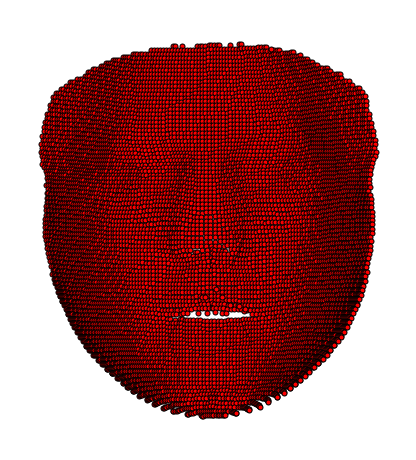
\includegraphics[valign=m,scale=0.16]{face_flow/images/3d_pca_basis/4_minus2}
    \end{tabular}%
    }
    \caption{The PCA basis of facial deformation learnt from the 
             3D LSFM~\cite{booth2016lsfm} model as described in 
             \cref{subsec:face_flow_experiments_basis}. The top and bottoms rows
             show the principals components for $\pm 2 \sigma$ respectively.}
\label{fig:face_flow_3d_pca_basis}
\end{figure}
\setlength{\tabcolsep}{6pt}
%%%%%%%%%%%%%%%%%%%%%%%%%%%%%%%%%%%%%%%%
%%%%%%%%%%%%%%%%%%%%%%%%%%%%%%%%%%%%%%%%
\setlength{\tabcolsep}{2pt}
\begin{figure}
    \centering
    \resizebox{\textwidth}{!}{%
    \begin{tabular}{cccccc}
    Mean &  PC 1 & PC 2 & PC 3 & PC 4 & PC 5 \\
    \multirow{2}{*}{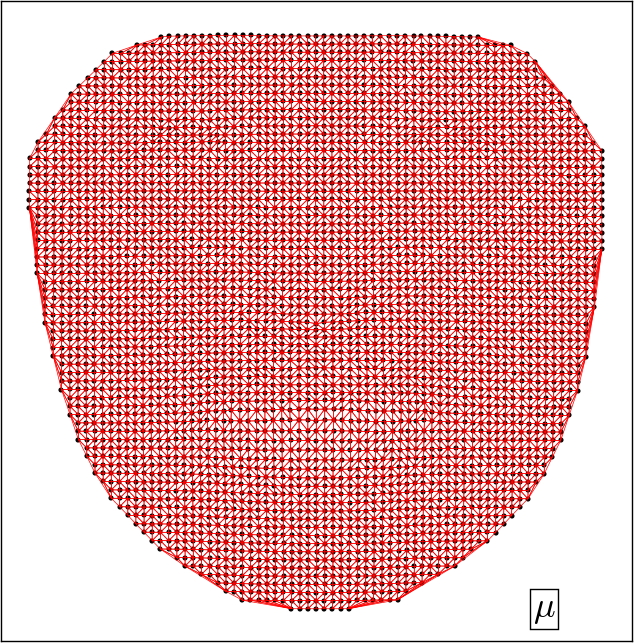
\includegraphics[valign=m,scale=0.16]{face_flow/images/of_pca_basis/mean}} &  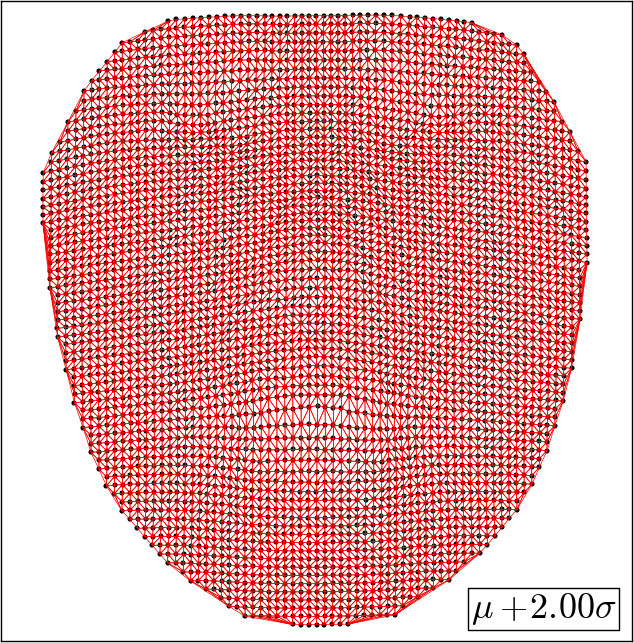
\includegraphics[valign=m,scale=0.16]{face_flow/images/of_pca_basis/0_plus2} & 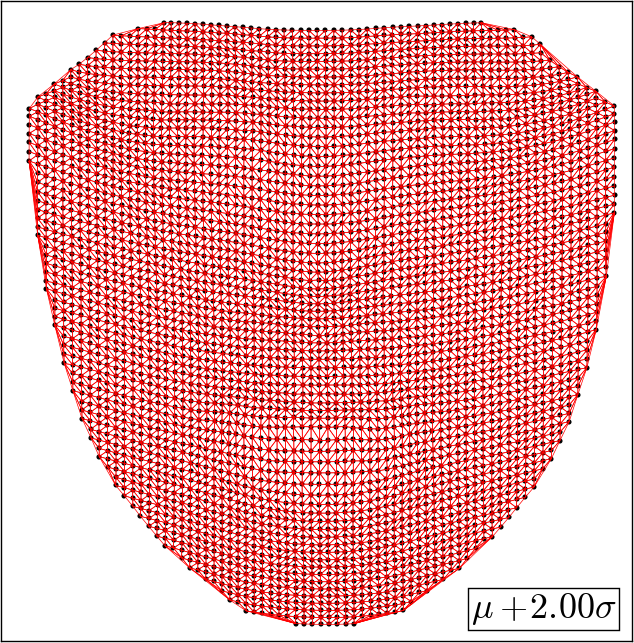
\includegraphics[valign=m,scale=0.16]{face_flow/images/of_pca_basis/1_plus2} & 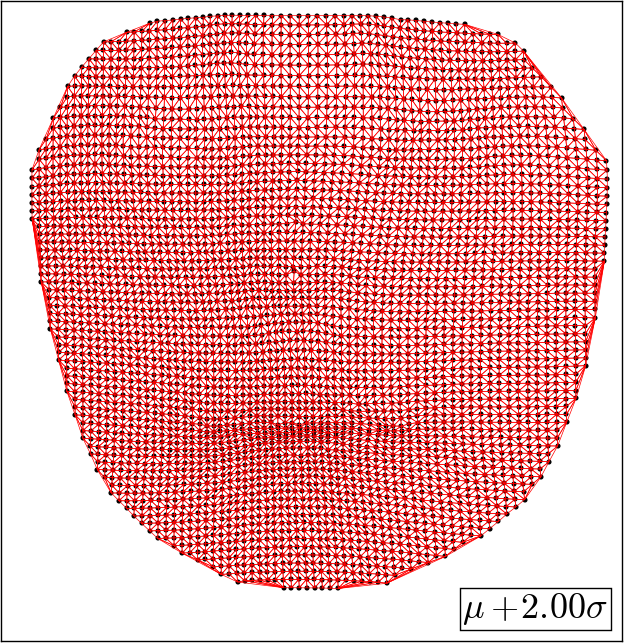
\includegraphics[valign=m,scale=0.16]{face_flow/images/of_pca_basis/2_plus2} & 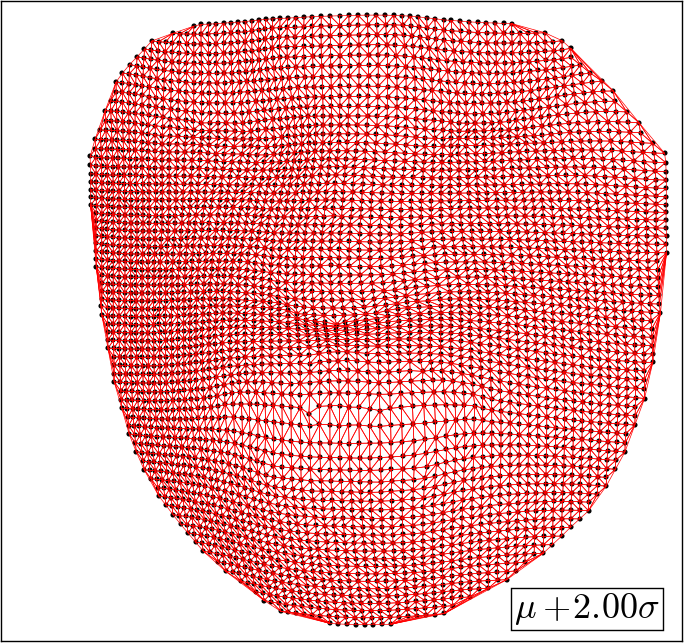
\includegraphics[valign=m,scale=0.16]{face_flow/images/of_pca_basis/3_plus2} & 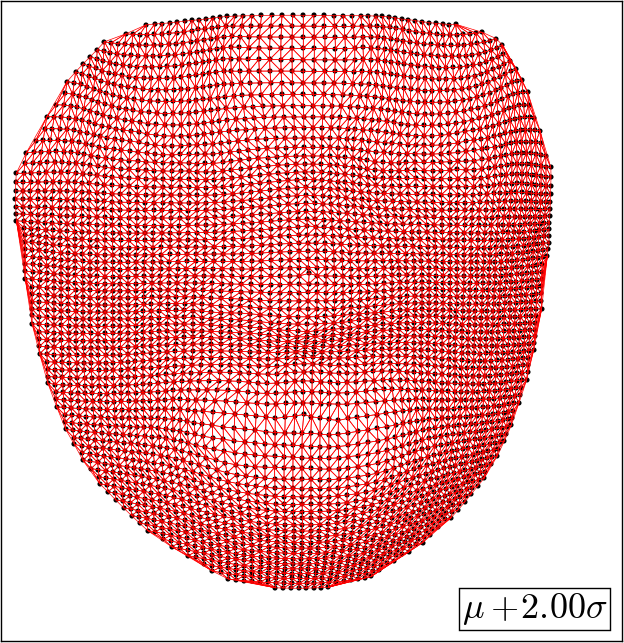
\includegraphics[valign=m,scale=0.16]{face_flow/images/of_pca_basis/4_plus2} \\
     & 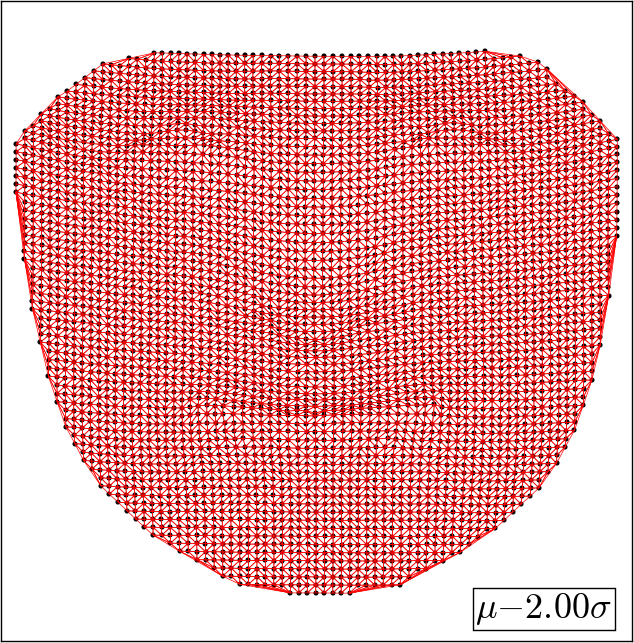
\includegraphics[valign=m,scale=0.16]{face_flow/images/of_pca_basis/0_minus2} & 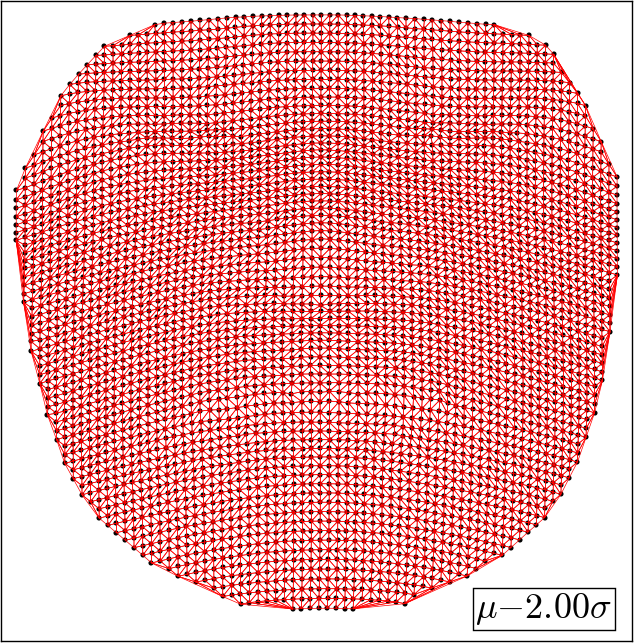
\includegraphics[valign=m,scale=0.16]{face_flow/images/of_pca_basis/1_minus2} & 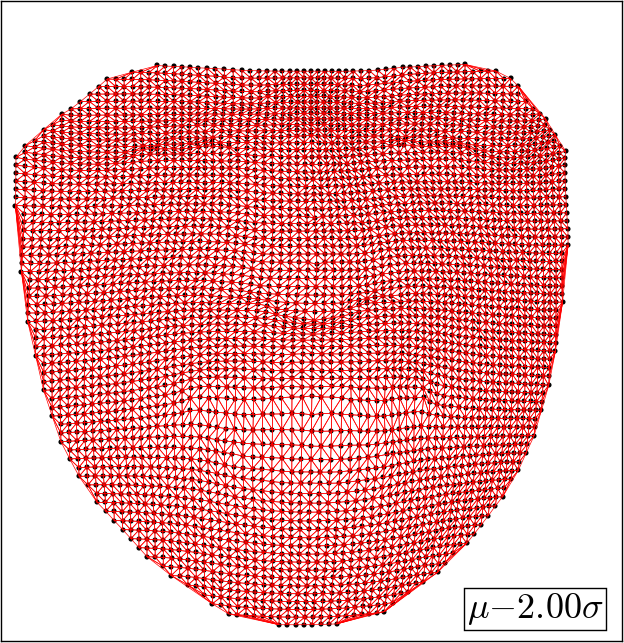
\includegraphics[valign=m,scale=0.16]{face_flow/images/of_pca_basis/2_minus2} & 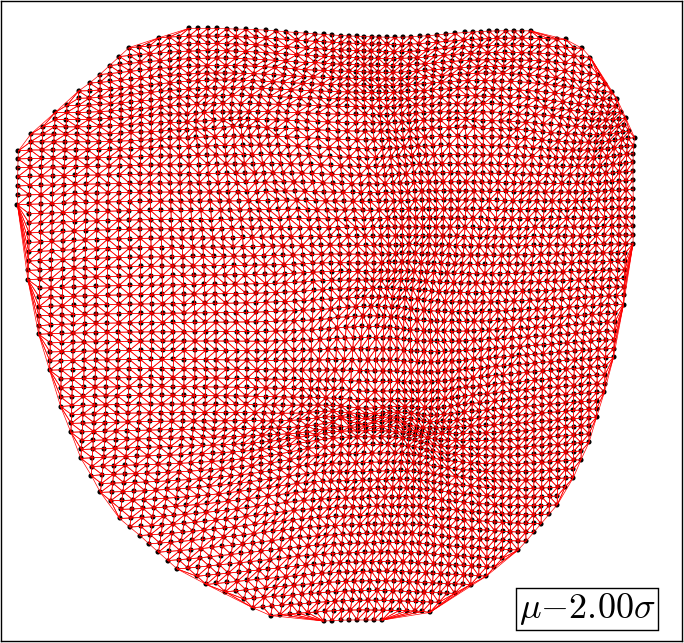
\includegraphics[valign=m,scale=0.16]{face_flow/images/of_pca_basis/3_minus2} & 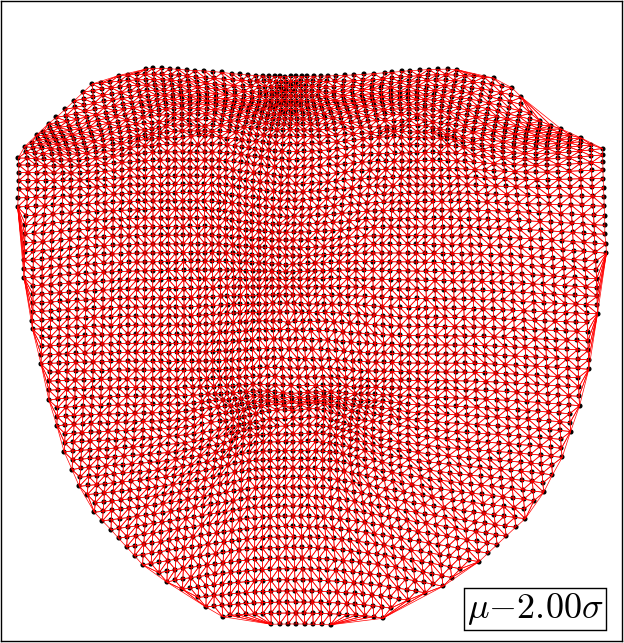
\includegraphics[valign=m,scale=0.16]{face_flow/images/of_pca_basis/4_minus2}
    \end{tabular}%
    }
    \caption{The PCA basis of facial deformation learnt from the 
             BU4D~\cite{yin2008high} database as described in 
             \cref{subsec:face_flow_experiments_basis}. The top and bottoms rows
             show the principals components for $\pm 2 \sigma$ respectively.}
\label{fig:face_flow_of_pca_basis}
\end{figure}
\setlength{\tabcolsep}{6pt}
%%%%%%%%%%%%%%%%%%%%%%%%%%%%%%%%%%%%%%%%
Our optical flow facial deformation basis is built by applying MFSF multi-frame optical flow method
\footnote{Code publicly available at https://bitbucket.org/troussos/mfsf/} of \citet{garg2013variational} on
the facial expression database BU4D~\cite{yin2008high}. We chose this database due
to the large range of expression present and the fact that is captured at a high
frame rate, which is ideal for the technique of \citet{garg2013variational}. However, in order
to further improve the performance of \citet{garg2013variational}, we augmented the energy
to include an extra quadratic landmark constraint. This landmark constraint
takes a similar form to the landmark constraint proposed in this paper, and was
found to improve the results considerably in sequences that displayed particularly
expressive emotion, such as surprise.

The BU4D database~\cite{yin2008high} consists of 102 subjects displaying 
6 canonical expression,
from neutral to the apex of the emotion. We selected a neutral frame for every
sequence and used this as the reference frame for the method of \citet{garg2013variational}.
After computing trajectories for each sequence,
we constructed a reference frame for our deformation basis using the mean
of the neutral images we selected previously. We then applied principal
component analysis (PCA) to learn the linear deformation model as described in 
\cref{sec:face_flow_learning_deformation}.
Experimentally, we found that $k=20$ principal components of
non-rigid deformation accounts for $~95\%$ of the variance.
We note that the BU4D-FE data shows frontal faces and thus our model does not capture out-of-plane
rotation. An illustration of the model is given in \cref{fig:face_flow_of_pca_basis}.

Our 3D statistical model was constructed by rendering instances from a modified
copy of the 3D morphable model provided by the 
Large Scale Facial Model (LSFM)~\cite{booth2016lsfm}. Only
the shape model was utilized in this work. We augmented this model by manually
aligning it with the mean blendshape model provided by 
FaceWarehouse~\cite{Cao:2014gy}. We then formed an additive linear model
of facial shape which allowed is to simulate expressions from the neutral
only data provided by the LSFM.\@ We then sampled 1000 instances
of this model within 2 standard deviations of the mean for LSFM and within a 
hand picked set of ranges for each blendshape. These blendshape values were
chosen in order to generate plausible facial shapes. These instances were
then rendered with 10 randomly generated 3D poses in the range $[-30, 30]$ for
the pitch and $[-60, 60]$ for the yaw. As described in
\cref{sec:face_flow_learning_deformation}, the occluded vertices were snapped
to the occluding contour. Standard 2D statistical model building procedure
was then followed and Procrustes analysis was performed and a PCA basis
constructed. An illustration of the model is given in \cref{fig:face_flow_3d_pca_basis}.
In these experiments, $~95\%$ of the variance is retained amounting to
$25$ components.
%%%%%%%%%%%%%%%%%%%%%%%%%%%%%%%%%%%%%%%%%%%%%%%%%%%%%%%%%%%%%%%%%%%%%%%%%%%%%%%%
\subsection{Optical Flow Basis: Motion Capture Data}\label{subsec:face_flow_experiments_mocap}
%%%%%%%%%%%%%%%%%%%%%%%%%%%%%%%%%%%%%%%%%%%%%%%%%%%%%%%%%%%%%%%%%%%%%%%%%%%%%%%%
%%%%%%%%%%%%%%%%%%%%%%%%%%%%%%%%%%%%%%%%%%%%%%%%%%%%%%%%%%%%%%%%%%%%%%%%%%%%%%%%
\begin{figure}
    \centering
    \begin{subfigure}{6in}
        \centering
        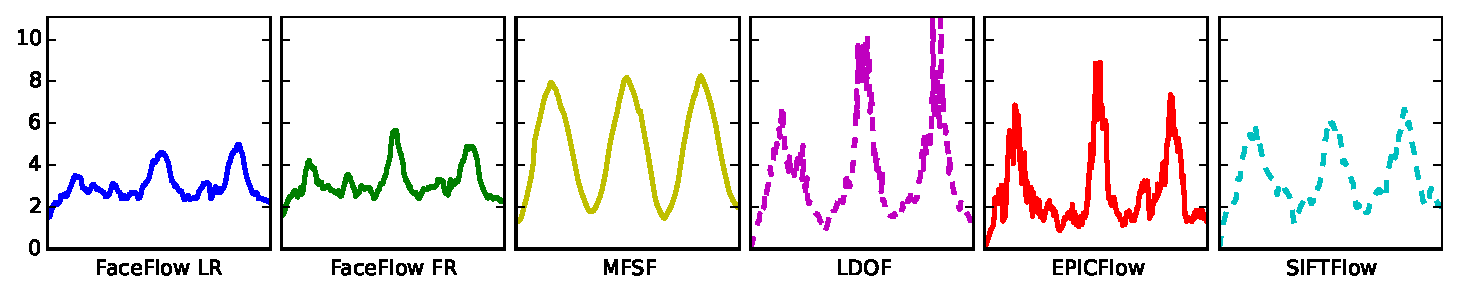
\includegraphics[width=\textwidth]{face_flow/images/synthetic/frame_error_5_flat}
    \end{subfigure}  \\
    \begin{subfigure}{6in}
        \centering
        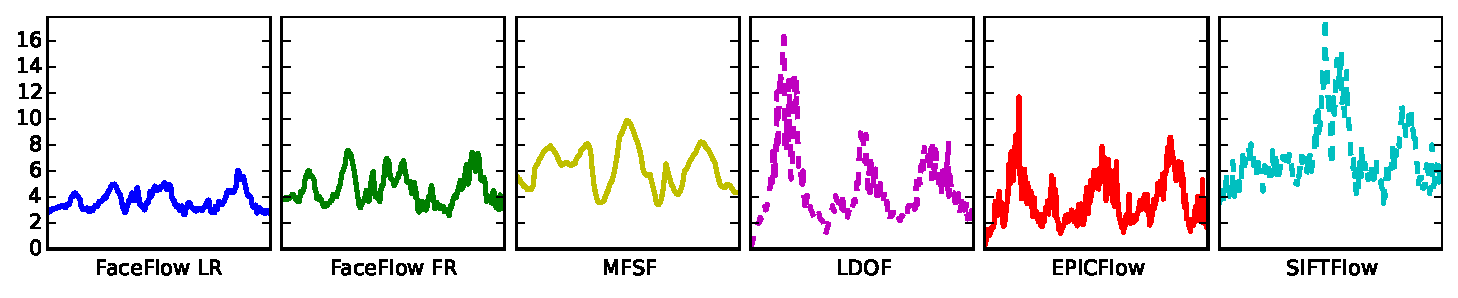
\includegraphics[width=\textwidth]{face_flow/images/synthetic/frame_error_6_flat}
    \end{subfigure}
    \caption{The average endpoint error calculated for each frame of the mocap
             sequence. Vertical axis is average endpoint error, horizontal is
             frame number. Top row is the illumination sequence, bottom row is
             illumination + occlusion.}
\label{fig:face_flow_per_frame_error}
\end{figure}
%%%%%%%%%%%%%%%%%%%%%%%%%%%%%%%%%%%%%%%%%%%%%%%%%%%%%%%%%%%%%%%%%%%%%%%%%%%%%%%%
In this experiment, we evaluated the performance of the optical flow basis
using a synthetic ground truth sequence. We use the performance capture 
dataset provided by \citet{zhang2004spacetime}
to generate three novel ground truth sequences consisting of 280 frames. 
This ground truth is provided by rendering
the sequence of meshes in a fixed pose, which yields both a texture and a set of vertices
in the scene. These vertices can then be used in order simply calculate flow for the face
throughout the image.

As mentioned, we rendered three sets of texture, all with the same underlying geometry,
to provide evidence of the robustness of Face Flow to challenging conditions. In the first
sequence, we rendered unmodified textures. This is a baseline
in order to show the performance of state-of-the-art methods for facial data. Since
our basis is trained using the output from~\cite{garg2013variational}, we do not expect to
outperform other optical flow techniques on this sequence. The second sequence
was rendered by rendering a periodically moving light source around the face. This
is challenging for the data term and helps to demonstrate the
robustness of our chosen feature descriptor. The final sequence is highly challenging. It contains
the periodic illumination variation from the previous sequence and also an artificial
occlusion in the form of a smoothly translating hand.

In order to initialise our Face Flow algorithm, we manually annotated the first frame
as the reference frame. To obtain an initial estimate of the coefficient
matrix $\mathbf{C}$, the landmark constraint quadratic term is solved, which
provides a reasonable estimate of the initial shape. Once solved in the reference frame,
this initialisation was propagated across every frame in the sequence. The landmark constraint
was otherwise not utilised in this experiment.

To evaluate the performance of the methods, we computed the root mean squared
error of the endpoints (RMSE), shown in \cref{tbl:face_flow_synthetic}. As expected
Face Flow does not outperform state-of-the-art methods in the original untampered
sequence. However, in the more interesting case of the illumination variation
and occlusion sequences, our Face Flow method with low-rank constraint (Face Flow LR),
performs the best. We also note that the low-rank method of our technique significantly
outperforms the full-rank version, particularly in the occluded sequence. 
Example endpoints for the three considered scenarios are given in 
\cref{fig:face_flow_synthetic_no_occl_examples,fig:face_flow_synthetic_illum_examples,%
fig:face_flow_synthetic_illum_occl_examples}. Note how
the face deformation is well localised and unlikely to undergo any gross deformations
due to being constrained by a statistical basis.

Finally, to provide evidence as to the stability of our algorithm, and the effect
of the low-rank constraint on the outcome of the sequence, we present 
\cref{fig:face_flow_per_frame_error}.
This figure shows the mean per-frame endpoint error across the sequence. The Face Flow
methods are given by the blue and green lines. Note how stable the Face Flow LR method is,
particularly when compared to the Face Flow FR method. We believe this effectively
demonstrates the positive effect enforcing soft temporal consistency can have.
%%%%%%%%%%%%%%%%%%%%%%%%%%%%%%%%%%%%%%%%%%%%%%%%%%%%%%%%%%%%%%%%%%%%%%%%%%%%%%%%
\begin{table}[t]
    \centering
    \begin{tabular}{cccccc}
                                                     \toprule
FF LR & FF FR & MFSF & LDOF & EPICFlow & SIFTFlow \\ \toprule
1.4   & 0.5   & 20   & 15   & $\sim$50 & 15       \\ \bottomrule
    \end{tabular}
    \caption{Run times \textit{per frame (in seconds)} for the 150 frame
             sequence shown in \cref{fig:face_flow_real_examples}. Images are
             $640\times480$. Performed on an Intel Xeon E5--1650 3.20GHz
             (32GB RAM). All times are approximate and averaged over multiple
             runs. EPICFlow times are dominated by
             DEEPMatching~\cite{weinzaepfel2013deepflow} ($~48$s).}
\label{tbl:face_flow_run_times}
\end{table}
%%%%%%%%%%%%%%%%%%%%%%%%%%%%%%%%%%%%%%%%%%%%%%%%%%%%%%%%%%%%%%%%%%%%%%%%%%%%%%%%
%%%%%%%%%%%%%%%%%%%%%%%%%%%%%%%%%%%%%%%%%%%%%%%%%%%%%%%%%%%%%%%%%%%%%%%%%%%%%%%%
\begin{table}
    \centering
    \begin{tabular}{lrrrrrr}
                                                                                                                                               \toprule
         & \multicolumn{2}{c}{Original}            & \multicolumn{2}{c}{Illumination}        & \multicolumn{2}{c}{Illumination + Occlusion} \\
         & {\scriptsize RMSE} & {\scriptsize AE95} & {\scriptsize RMSE} & {\scriptsize AE95} & {\scriptsize RMSE} & {\scriptsize AE95}      \\ \toprule
FF LR    & 2.95               & 5.52               & {\bf 3.56}         & {\bf 6.63}         & {\bf 4.48}         & {\bf 8.47}              \\
FF FR    & 3.24               & 6.01               & 3.76               & 7.02               & 5.83               & 11.50                   \\
MFSF     & 1.73               & 3.20               & 6.33               & 13.68              & 8.25               & 17.30                   \\
LDOF     & {\bf 1.56}         & {\bf 2.79}         & 4.84               & 9.98               & 6.54               & 11.44                   \\
EPICFlow & 1.66               & 3.25               & 4.02               & 9.61               & 5.15               & 11.61                   \\
SIFTF    & 2.65               & 5.15               & 4.89               & 11.81              & 11.82              & 23.05                   \\ \bottomrule
    \end{tabular}
    \caption{RMSE and 95\% average endpoint error for the synthetic data.}
\label{tbl:face_flow_synthetic}
\end{table}
%%%%%%%%%%%%%%%%%%%%%%%%%%%%%%%%%%%%%%%%%%%%%%%%%%%%%%%%%%%%%%%%%%%%%%%%%%%%%%%%
%%%%%%%%%%%%%%%%%%%%%%%%%%%%%%%%%%%%%%%%%%%%%%%%%%%%%%%%%%%%%%%%%%%%%%%%%%%%%%%%
\begin{landscape}
\thispagestyle{footeronly}
\setlength{\tabcolsep}{1pt}
\begin{figure}[t]
    \centering
    \begin{tabular}{ccccccccc}
           & Frame & Ground Truth & FF LR & FF FR & MFSF & LDOF & EPICFlow & SIFTFlow \\ \vspace{-0.3cm}
        16 & \framerowsynth{nonoccluded}{16}   \\ \vspace{-0.3cm}
        54 & \framerowsynth{nonoccluded}{54}    \\ \vspace{-0.3cm}
        139 & \framerowsynth{nonoccluded}{139} \\
        233 & \framerowsynth{nonoccluded}{233}
    \end{tabular}
    \caption{Example endpoint results for the original synthetic sequence 
             without any outliers. Each row shows a different 
             frame of the 280 frame synthetic sequence (Frame 16, 54, 139 and 
             233 from top to bottom)}
\label{fig:face_flow_synthetic_no_occl_examples}
\end{figure}
\setlength{\tabcolsep}{6pt}
\end{landscape}
%%%%%%%%%%%%%%%%%%%%%%%%%%%%%%%%%%%%%%%%%%%%%%%%%%%%%%%%%%%%%%%%%%%%%%%%%%%%%%%%
%%%%%%%%%%%%%%%%%%%%%%%%%%%%%%%%%%%%%%%%%%%%%%%%%%%%%%%%%%%%%%%%%%%%%%%%%%%%%%%%
\begin{landscape}
\thispagestyle{footeronly}
\setlength{\tabcolsep}{1pt}
\begin{figure}[t]
    \centering
    \begin{tabular}{ccccccccc}
           & Frame & Ground Truth & FF LR & FF FR & MFSF & LDOF & EPICFlow & SIFTFlow \\ \vspace{-0.3cm}
        16 & \framerowsynth{illumination}{16}    \\ \vspace{-0.3cm}
        54 & \framerowsynth{illumination}{54}    \\ \vspace{-0.3cm}
        139 & \framerowsynth{illumination}{139}  \\
        233 & \framerowsynth{illumination}{233}
    \end{tabular}
    \caption{Example endpoint results for the synthetic sequence including
             illumination variation. Each row shows a different frame of the
             280 frame synthetic sequence (Frame 16, 54, 139 and 233 from top
             to bottom)}
\label{fig:face_flow_synthetic_illum_examples}
\end{figure}
\setlength{\tabcolsep}{6pt}
\end{landscape}
%%%%%%%%%%%%%%%%%%%%%%%%%%%%%%%%%%%%%%%%%%%%%%%%%%%%%%%%%%%%%%%%%%%%%%%%%%%%%%%%
%%%%%%%%%%%%%%%%%%%%%%%%%%%%%%%%%%%%%%%%%%%%%%%%%%%%%%%%%%%%%%%%%%%%%%%%%%%%%%%%
\begin{landscape}
\thispagestyle{footeronly}
\setlength{\tabcolsep}{1pt}
\begin{figure}[t]
    \centering
    \begin{tabular}{ccccccccc}
           & Frame & Ground Truth & FF LR & FF FR & MFSF & LDOF & EPICFlow & SIFTFlow \\ \vspace{-0.3cm}
        16 & \framerowsynth{illumination_occlusion}{16}    \\ \vspace{-0.3cm}
        54 & \framerowsynth{illumination_occlusion}{54}    \\ \vspace{-0.3cm}
        139 & \framerowsynth{illumination_occlusion}{139}  \\
        233 & \framerowsynth{illumination_occlusion}{233}
    \end{tabular}
    \caption{Example endpoint results for the synthetic sequence including
             illumination and occlusion variation. Each row shows a different 
             frame of the 280 frame synthetic sequence (Frame 16, 54, 139 and 
             233 from top to bottom)}
\label{fig:face_flow_synthetic_illum_occl_examples}
\end{figure}
\setlength{\tabcolsep}{6pt}
\end{landscape}
%%%%%%%%%%%%%%%%%%%%%%%%%%%%%%%%%%%%%%%%%%%%%%%%%%%%%%%%%%%%%%%%%%%%%%%%%%%%%%%%
%%%%%%%%%%%%%%%%%%%%%%%%%%%%%%%%%%%%%%%%%%%%%%%%%%%%%%%%%%%%%%%%%%%%%%%%%%%%%%%%
\begin{landscape}
\thispagestyle{footeronly}
\newcommand{\framerowreal}[1]{%
\adjustbox{valign=m,vspace=1pt}{\includegraphics[width=4.5cm,height=3.45cm]{face_flow/images/real/#1_ff_dsift_sequence}} &
\adjustbox{valign=m,vspace=1pt}{\includegraphics[width=4.5cm,height=3.45cm]{face_flow/images/real/#1_mfsf}}              &
\adjustbox{valign=m,vspace=1pt}{\includegraphics[width=4.5cm,height=3.45cm]{face_flow/images/real/#1_ldof}}              &
\adjustbox{valign=m,vspace=1pt}{\includegraphics[width=4.5cm,height=3.45cm]{face_flow/images/real/#1_epicflow}}          &
\adjustbox{valign=m,vspace=1pt}{\includegraphics[width=4.5cm,height=3.45cm]{face_flow/images/real/#1_siftflow}}
}

\setlength{\tabcolsep}{1pt}
\begin{figure}[t]
    \centering
    \begin{tabular}{cccccc}
           & Face Flow LR & MFSF & LDOF & EPICFlow & SIFTFlow \\ \vspace{-0.1cm}
        15 & \framerowreal{15}                                \\ \vspace{-0.1cm}
        21 & \framerowreal{21}                                \\ \vspace{-0.1cm}
       119 & \framerowreal{119}
    \end{tabular}
    \caption{Results on real data. Here, we incorporate the landmark constraint
             and thus do not give results for Face Flow FR.}
\label{fig:face_flow_real_examples}
\end{figure}
\setlength{\tabcolsep}{6pt}
\end{landscape}
%%%%%%%%%%%%%%%%%%%%%%%%%%%%%%%%%%%%%%%%%%%%%%%%%%%%%%%%%%%%%%%%%%%%%%%%%%%%%%%%
%%%%%%%%%%%%%%%%%%%%%%%%%%%%%%%%%%%%%%%%%%%%%%%%%%%%%%%%%%%%%%%%%%%%%%%%%%%%%%%%
\subsection{Optical Flow Basis: ``In-the-wild'' Sequence}\label{subsec:face_flow_experiments_real}
%%%%%%%%%%%%%%%%%%%%%%%%%%%%%%%%%%%%%%%%%%%%%%%%%%%%%%%%%%%%%%%%%%%%%%%%%%%%%%%%
In this experiment, we evaluated the performance of the optical flow basis
using a challenging ``in-the-wild'' sequence.
The sequence consisting of 150 frames of a young woman reacting to a video. 
She reacts negatively and clearly presents discomfort by touching her face and shifting
in her seat. This amounts to challenging variation in the sequence, including
occlusions from her hand and motion blur from movement. In this sequence,
we also provide evidence as to the benefit of incorporating the landmark constraint. The sequence was
automatically landmarked using~\cite{kazemi2014one}, then our method was initialised with
these landmarks for every frame. We also used the landmarks for the quadratic penaliser term.
As \cref{fig:face_flow_real_examples} shows, Face Flow LR performs very well in this sequence. 
In particular, we note that our method is very robust to the presence of occlusions, 
aided by the sparse landmarks provided by~\cite{kazemi2014one}. 
We also provide \cref{tbl:face_flow_run_times}
which demonstrates that Face Flow is an order of magnitude more efficient than
the other considered methods for this sequence.
%%%%%%%%%%%%%%%%%%%%%%%%%%%%%%%%%%%%%%%%%%%%%%%%%%%%%%%%%%%%%%%%%%%%%%%%%%%%%%%%
\subsection{3D Projected Basis: ``In-the-wild'' Sequence}\label{subsec:face_flow_experiments_boris}
%%%%%%%%%%%%%%%%%%%%%%%%%%%%%%%%%%%%%%%%%%%%%%%%%%%%%%%%%%%%%%%%%%%%%%%%%%%%%%%%
%%%%%%%%%%%%%%%%%%%%%%%%%%%%%%%%%%%%%%%%%%%%%%%%%%%%%%%%%%%%%%%%%%%%%%%%%%%%%%%%
\begin{figure}
    \centering
    \hspace*{\fill}
    \begin{subfigure}[b]{0.163\textwidth}
        \centering
        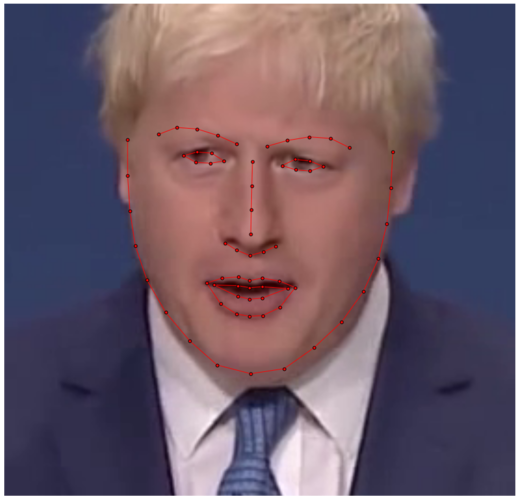
\includegraphics[width=\textwidth]{face_flow/images/boris/boris_template}
        \caption*{Template Frame}
    \end{subfigure}  \hfill
    \begin{subfigure}[b]{0.23\textwidth}
        \centering
        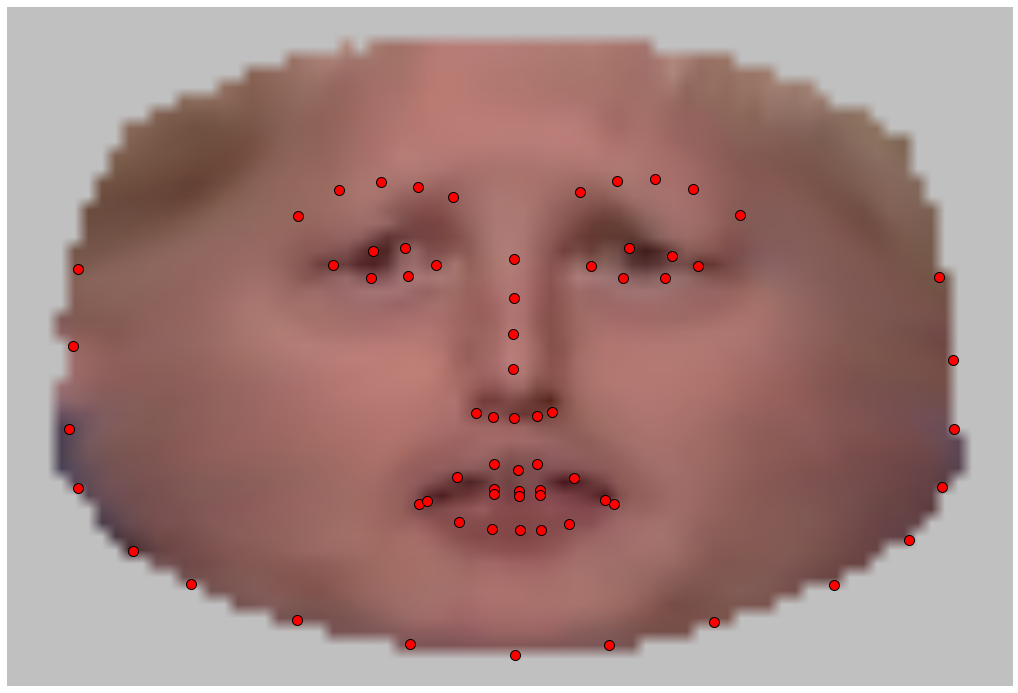
\includegraphics[width=\textwidth]{face_flow/images/boris/boris_sampled_template_05}
        \caption*{$0.5\times$ Highest Resolution}
    \end{subfigure}  \hfill
    \begin{subfigure}[b]{0.23\textwidth}
        \centering
        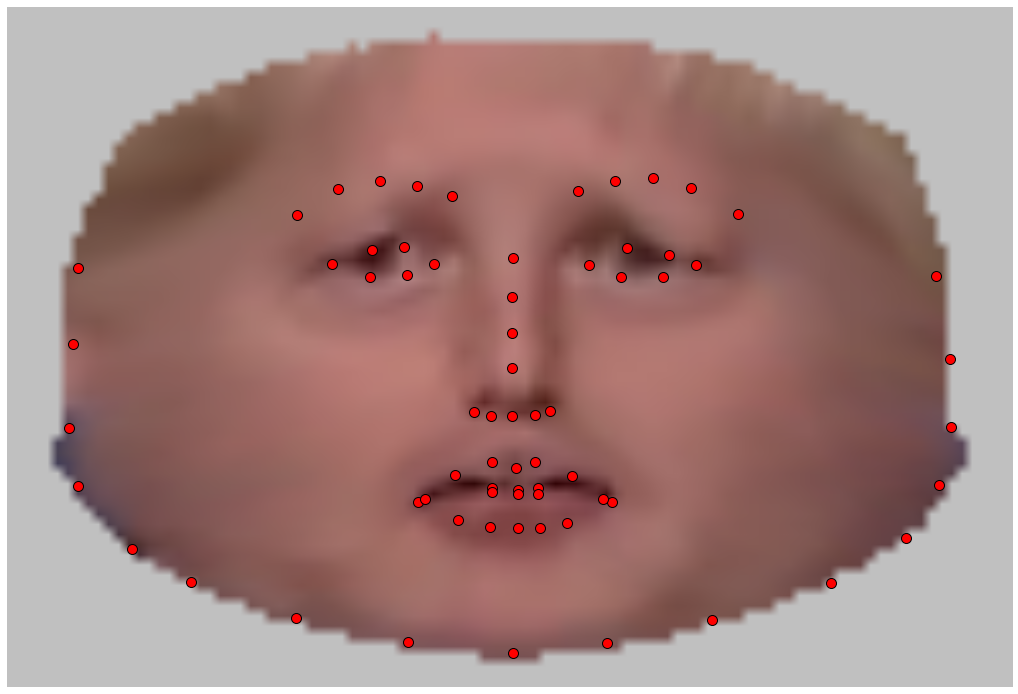
\includegraphics[width=\textwidth]{face_flow/images/boris/boris_sampled_template_07}
        \caption*{$0.7\times$ Highest Resolution}
    \end{subfigure}  \hfill
    \begin{subfigure}[b]{0.23\textwidth}
        \centering
        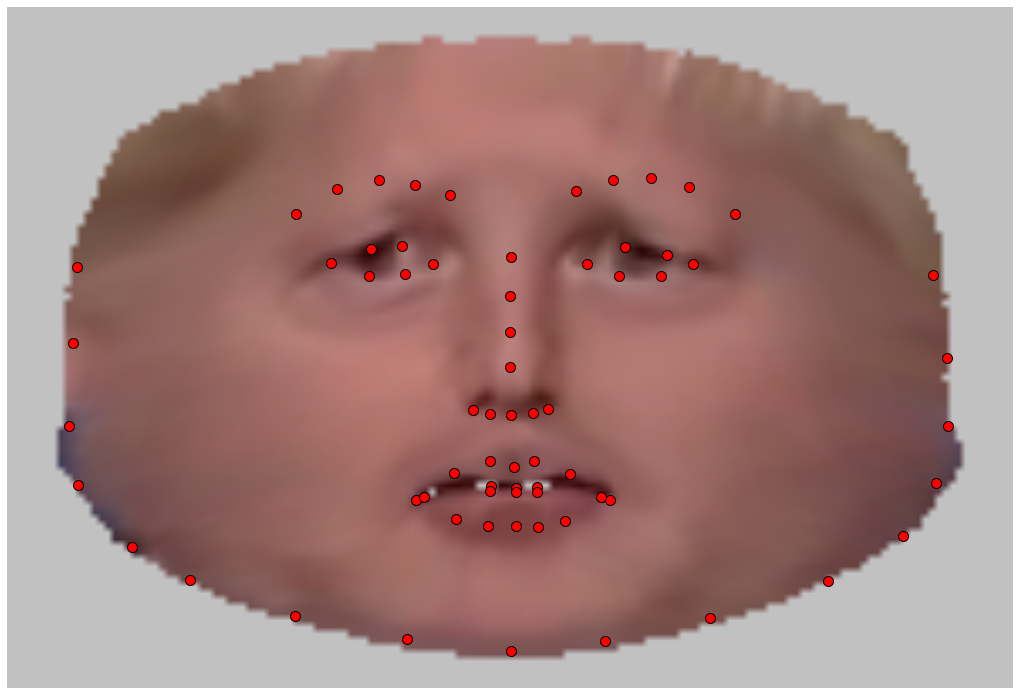
\includegraphics[width=\textwidth]{face_flow/images/boris/boris_sampled_template_10}
        \caption*{Highest Resolution}
    \end{subfigure}
    \hspace*{\fill}
    \caption{The template frame and the it's three scales built from the
             ``in-the-wild'' sequence of Boris Johnson. From left to right
             the templates increase in resolution, with the furthest right being
             the highest resolution used for fitting, with a diagonal of
             approximately 150 pixels.}
\label{fig:face_flow_boris_references}
\end{figure}
%%%%%%%%%%%%%%%%%%%%%%%%%%%%%%%%%%%%%%%%%%%%%%%%%%%%%%%%%%%%%%%%%%%%%%%%%%%%%%%%
In this experiment we qualitatively evaluate the performance of our basis
built from the 3D statistical model. In particular, we provide results on
an expressive sequence of the politician Boris Johnson giving a speech, taken
from one of training videos of the 
300-VW competition~\cite{Chrysos:2015gt,shen2015first}. This sequence consists
of 100 frames and contains out-plane rotation and expressive speaking. We
consider this a suitable sequence for evaluating the 3D projected model
as it demonstrates the Face Flow can handle out-of-plane rotations when
given a properly trained deformation basis. It also demonstrates the quality
of the 3D reconstruction recovered in comparison to using only the sparse
68 points provided by \citet{shen2015first}. Other than the change of deformation
basis, all other parameters were maintained.

To build the Face Flow template, the closest to neutral frame in the sequence 
was chosen and warped by performing the least squares fitting on the 68 
points described in \cref{sec:face_flow_3d_recovery}. 
\cref{fig:face_flow_boris_references} shows the 3 references frames from 
the multi-scale Face Flow model. For qualitative comparison we compare the result
of recovering the 3D statistical parameters from the dense points recovered by
face flow from the sparse 68 points originally provided by the 300-VW competition.
Similar to the experiment in \cref{subsec:face_flow_experiments_real}, we do
utilize the sparse landmarks constraint with a weight of $0.05$. 
\cref{fig:face_flow_boris_results} shows the results of the Face Flow recovery
against only fitting the sparse 68 points. The dense 2D fitting column refers
the result of Face Flow. In the case of the sparse results, the dense fitting
refers to fitting the 68 sparse points of the 2D deformation basis. This
rendering is provided in order to show the expressiveness of the 2D deformation
basis with respect to manually annotated landmarks.

In order to recover the 3D results, the non-linear problem described in
\cref{sec:face_flow_3d_recovery} is solved. For Face Flow, this is solved densely
on all of the points returned by Face Flow. For the sparse points, only the 68
points are discovered. The furthest right column, which shows the 3D renderings,
gives the clearest view of the results. It clearly shows that simply fitting
the sparse points can cause the recovered 3D surface to resemble a caricature. 
We also note that the results from Face Flow appear more consistent and more
closely resemble the same individual, which we propose is likely due to the
low-rank constraint constraining the output of the 2D deformations.
Despite this low-rank constraint, the results still closely match the expression
and appear more accurate than the fitting from the sparse points.
However, the Face Flow fitting does have issues with fitting the boundaries of
the face and often underestimates the extent of the cheek areas.
%%%%%%%%%%%%%%%%%%%%%%%%%%%%%%%%%%%%%%%%%%%%%%%%%%%%%%%%%%%%%%%%%%%%%%%%%%%%%%%%
\begin{table}[t]
    \centering
    \resizebox{\textwidth}{!}{%
        \begin{tabular}{c|cccc}
        \toprule
        Input Frame & Initialisation & Dense 2D Fitting & Rasterizion & Rendering \\ \midrule
        \framerowboris{0}{3}{1.6}  \\ \midrule
        \framerowboris{77}{3}{1.6} \\ \midrule
        \framerowboris{94}{3}{1.6} \\
        \bottomrule
    \end{tabular}%
    }
    \caption{Results from the Boris Johnson sequence. Each row is a different
             frame. The top inner row of each result row are from the dense
             fitting of Face Flow. The bottom row is the result of solving 
             the least squares problem on the 68 points shown in the input
             frame column. The initialisation column refers to the lowest
             resolution initialisation used for fitting Face flow. The dense 2D
             fitting refers to the result of Face Flow and the result of fitting
             the 68 points to the 2D deformation basis.}
\label{fig:face_flow_boris_results}
\end{table}
%%%%%%%%%%%%%%%%%%%%%%%%%%%%%%%%%%%%%%%%%%%%%%%%%%%%%%%%%%%%%%%%%%%%%%%%%%%%%%%%
